\newpage
\section{Implementation 2}
\label{implementation_2}
\subsection{Opening Distance}
The gripper opening in simulation is controlled based on the position of the motor of the exoskeleton. The motor position when the exoskeleton is closed is 5$^{\circ}$, and when the exoskeleton is fully open, 205$^{\circ}$. The rack and pinion mechanism is designed in a way that less than a full rotation is needed to fully open the gripper, so there is no ambiguity between the positions. The gripper opening in simulation is calculated by multiplying the normalized exoskeleton opening by the range of the gripper in simulation.

\begin{equation}
d_{\text{gripper}} = \frac{p_{\text{motor}} - p_{\text{min}}}{p_{\text{max}} - p_{\text{min}}} \cdot R_{\text{gripper}}
\end{equation}

\noindent
where:
\begin{itemize}
\item \( R_{\text{gripper}} = 0.127 \) is the maximum gripper opening range (simulation distance units),
\item \( p_{\text{min}} = 5 \) and \( p_{\text{max}} = 205 \) are the motor position limits (degrees),
\item \( p_{\text{motor}} \) is the current motor position,
\item \( d_{\text{gripper}} \) is the computed gripper opening. 
\end{itemize}

\subsection{Force}

\noindent
When the gripper closes around the soft ball, the soft ball provides normal reaction forces $R_l$ and $R_r$ (Fig. \ref{fig:pybullet_getContactPoints}). The motor is driven using the current control operation mode. The process to calculate the goal current has multiple steps. Firstly, the forces are summed to obtain the total force.

\begin{equation}
F_{\text{total}} = R_l + R_r
\end{equation}

\noindent
Then rearranging Eq. \ref{eq:rack_and_pinnion_force}, theoretical torque is obtained (Eq. \ref{eq:rack_and_pinnion_theoretical_torque}).

\begin{equation}
\tau_m = F_{\text{total}} \cdot r_p
\label{eq:rack_and_pinnion_theoretical_torque}
\end{equation}

\noindent
By taking into account the efficiency of the system, the required torque is obtained.

\begin{equation}
\tau_{\text{applied}} = \frac{\tau_m}{0.5693}
\label{eq:applied_torque_final}
\end{equation}

\noindent
Exponential smoothing with window size 10 is applied, the same as with \nameone, to obtain the final goal torque. Then this goal torque is converted to the motor's goal current Eq. \ref{eq:applied_goal_current_2}.

\begin{equation}
I_{\text{goal}} = \frac{\tau_{\text{goal}}}{k_t}
\label{eq:applied_goal_current_2}
\end{equation}

\noindent
The motor's goal current registry accepts an integer. The final transformation is to quantize the goal current using the motor's current unit of 2.69 [mA] (Eq. \ref{eq:applied_goal_current_quantized}).

\begin{equation}
I_{\text{quantized}} = \operatorname{round} \left( \frac{I_{\text{goal}}}{2.69e^{-3}} \right)
\label{eq:applied_goal_current_quantized}
\end{equation}

\noindent
Using these equations in the softball squeezing testing environment (Fig. \ref{fig:pybullet_env_design_one}), a force graph is obtained (Fig. \ref{fig:force_graph_results_ball_squeezing_design_2}).

\begin{figure}[ht]
\centering
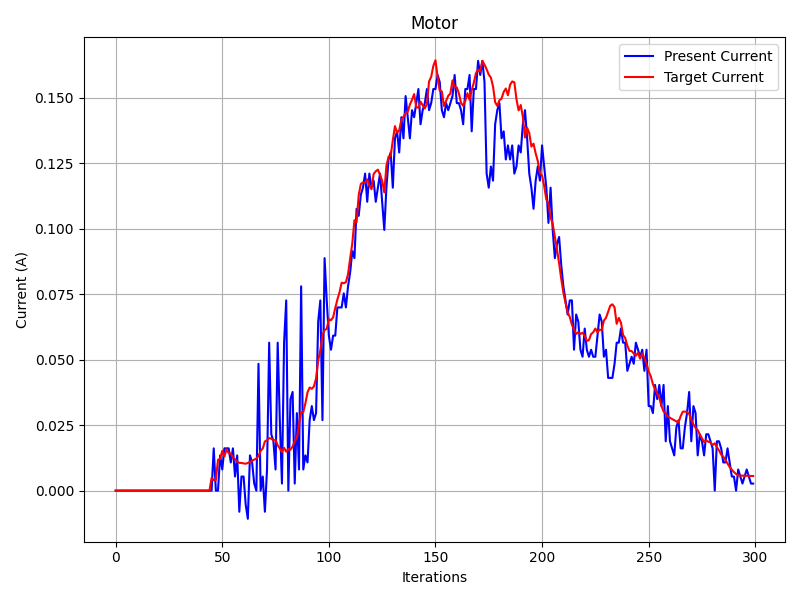
\includegraphics[width=0.8\linewidth]{chapters/exoskeleton/images/implementation2/squeeze_test_results.png}
\caption{Squeezing soft virtual ball with target current smoothing window K=10 using \nametwo}
\label{fig:force_graph_results_ball_squeezing_design_2}
\end{figure}

\subsection{Tracking}
The goal position for the tracking is obtained by capturing the VR controller's pose and applying a fixed transformation to account for the physical offset between the controller (located on the back of the hand) and the exoskeleton. An issue arises when setting the goal position directly in the simulation every frame: the gripper passes through the virtual objects, and the user is not able to interact with them.

\noindent
To overcome this issue, a proportional (P) controller is employed based on positional and orientational errors. Controlling the gripper through linear and angular velocities instead of directly setting the position allows the gripper to interact and collide with virtual objects. The positional error definition is shown in Eq. \ref{eq:pos_error_gripper_2}. 

\begin{equation} e_p = p_{target} - p_{current} \label{eq:pos_error_gripper_2} \end{equation}

\noindent
From this error, the corresponding target linear velocity is computed using Eq. \ref{eq:v_linear_gripper_2}.

\begin{equation} v_{linear} = K_p \cdot e_p \label{eq:v_linear_gripper_2} \end{equation}

\noindent
For orientation control, the orientational error is computed using the quaternion difference Eq. \ref{eq:or_error_gripper_2}.

\begin{equation} e_o = q_{target} \cdot q_{current}^{-1} \label{eq:or_error_gripper_2} \end{equation}

\noindent
The quaternion error $e_o$ represents the relative rotation needed to align the current orientation with the target. A quaternion consists of a scalar part and a vector part \cite{siciliano2010robotics}. The target angular velocity is then obtained by scaling the vector part with a proportional gain (Eq. \ref{eq:v_angular_gripper_2}).

\begin{equation} v_{angular} = K_o \cdot (e_{o,x}, e_{o,y}, e_{o,z}) \label{eq:v_angular_gripper_2} \end{equation}

\noindent
Eq. \ref{eq:v_angular_gripper_2} is just an approximation, and a deeper explanation is needed in order to understand why it works. The quaternion can be written as (Eq. \ref{eq:expanded_quaternion_form}):

\begin{equation} q = [w, x, y, z] = \left[ \cos\left(\frac{\theta}{2}\right), \sin\left(\frac{\theta}{2}\right) n \right] \label{eq:expanded_quaternion_form} \end{equation}

where:
\begin{itemize}
\item \( \theta \) is the angle of rotation.
\item \( n \) is the unit vector along the axis of rotation.
\end{itemize}

\noindent
Ideally the angular velocity using a proportional (P) controller would be calculated based on this axis-angle representation (Eq. \ref{eq:ideal_v_angular_gripper_2}).

\begin{equation} v_{angular} = K_o \cdot \theta n \label{eq:ideal_v_angular_gripper_2} \end{equation}

\noindent
The axis and angle can be calculated from the quaternion directly (Eq. \ref{eq:axis_and_angle_calculation}).

\begin{equation}
\label{eq:axis_and_angle_calculation}
\begin{aligned}
n &= \frac{[x, y, z]}{\sin(\theta/2)} \\
\theta &= 2 \cos^{-1}(w)
\end{aligned}
\end{equation}

\noindent
The problem with this approach (besides requiring more computation) is that if the rotational error is small, the axis will be undefined. This does not work for the desired case, as the goal of the proportional controller is to minimize the error to zero. That's why small angle approximation is used (Eq. \ref{eq:small_angle_approximation}).

\begin{equation} \sin\left(\frac{\theta}{2}\right) \approx \frac{\theta}{2} \label{eq:small_angle_approximation} \end{equation}

\noindent
Thus the Eq. \ref{eq:v_angular_gripper_2} using small angle approximation becomes Eq. \ref{eq:small_angle_approximation_angular_velocity}.

\begin{equation} v_{angular} = K_o \cdot \sin\left(\frac{\theta}{2}\right)n \approx  K_o \cdot \frac{\theta}{2}n \label{eq:small_angle_approximation_angular_velocity} \end{equation}

\noindent
Now it should be clear how the implemented angular velocity controller Eq. \ref{eq:v_angular_gripper_2} and ideal Eq. \ref{eq:ideal_v_angular_gripper_2} are related. The implemented controller does need a higher gain $K_o$ as it has division by two implicitly absorbed into it. Due to the approximation, the system is no longer linear. The PyBullet implementation has high-frequency updates, resulting in small orientation errors. This allows the error to converge towards zero, resulting in a system capable of tracking the pose of the exoskeleton in VR and enabling interaction with virtual objects.
